% Gemini theme
% See: https://rev.cs.uchicago.edu/k4rtik/gemini-uccs
% A fork of https://github.com/anishathalye/gemini

\documentclass[final]{beamer}

% ====================
% Packages
% ====================
\usepackage{amsfonts}
\usepackage[T1]{fontenc}
\usepackage{lmodern}
\usepackage[size=custom,width=120,height=72,scale=1.0]{beamerposter}
\geometry{paperwidth=48in,paperheight=36in}
\usetheme{gemini}
\usecolortheme{ucf}
\usepackage{graphicx}
\usepackage{booktabs}
\usepackage{tikz}
\usepackage{pgfplots}
\pgfplotsset{compat=1.14}

\usepackage{float}
\usepackage{xspace}
\usepackage{graphicx}
\graphicspath{{./imgs/}}
\usepackage{comment}
\usepackage{listings,hyperref}
\usepackage{cite}

% nice looking audit titles
\newcommand{\Minerva}{\textsc{Minerva}\xspace}
\newcommand{\Prov}{\textsc{Providence}\xspace}
\newcommand{\B}{{{B2}}\xspace}
\newcommand{\R}{{{R2}}\xspace}
\newcommand{\BRAVO}{\textsc{BRAVO}\xspace}


% ====================
% Lengths
% ====================

% If you have N columns, choose \sepwidth and \colwidth such that
% (N+1)*\sepwidth + N*\colwidth = \paperwidth
\newlength{\sepwidth}
\newlength{\colwidth}
\setlength{\sepwidth}{0.001\paperwidth}
\setlength{\colwidth}{0.23\paperwidth}

\newcommand{\separatorcolumn}{\begin{column}{\sepwidth}\end{column}}

% ====================
% Title
% ====================

\title{Election Security with Risk-Limiting Audits}

%\author{Nitish A. Gupta \inst{1} \and Nitish A. Gupta \inst{2}}
\author{Oliver Broadrick\inst{1} \and
Poorvi L. Vora\inst{1} \and
Filip Zag{\'o}rski\inst{2}\inst{3}}
% First names are abbreviated in the running head.
% If there are more than two authors, 'et al.' is used.
%
\institute[shortinst]{\inst{1} Department of Computer Science, The George Washington University%\thanks{Supported in part by NSF Award 2015253} 
\samelineand \inst{2} Wroclaw University of Science and Technology%\thanks{Author was partially supported by Polish National Science Centre contract number DEC-2013/09/D/ST6/03927} and 
\samelineand \inst{3} Votifica
}
%

%\institute[shortinst]{\inst{1} \textit{University of Central Florida, Orlando, FL} \samelineand \inst{2} Another Institute}

% ====================
% Footer (optional)
% ====================

\footercontent{
  \href{odbroadrick@gmail.com}{odbroadrick@gmail.com}
}
% (can be left out to remove footer)

% ====================
% Logo (optional)
% ====================

% use this to include logos on the left and/or right side of the header:
% \logoright{\includegraphics[height=7cm]{logo1.pdf}}
% \logoleft{\includegraphics[height=7cm]{logo2.pdf}}

% ====================
% Body
% ====================

\begin{document}
\addtobeamertemplate{headline}{}
{
    \begin{tikzpicture}[remember picture,overlay]
      \node [anchor=north west, inner sep=3cm] at ([xshift=0.0cm,yshift=3cm]current page.north west)
      {
\includegraphics[height=8cm]{logos/gw.png}}; % also try shield-white.eps
      \node [anchor=north east, inner sep=3cm] at ([xshift=0.0cm,yshift=3cm]current page.north east)
      {
\includegraphics[height=8cm]{logos/gw.png}};
    \end{tikzpicture}
}

\begin{frame}[t]
\begin{columns}[t]
\separatorcolumn

\begin{column}{\colwidth}

\begin{block}{Risk-Limiting Audits}
\begin{itemize}
\item
In election security, a risk-limiting audit (RLA) draws trusted paper ballots in rounds, stopping if a rigorous statistical criterion is satisfied, or proceeding to a full hand count. If the announced outcome of the election is erroneous, an RLA will detect the error with high, predetermined minimum probability. 

\item
An audit $\mathcal{A}$ takes a sample of ballots $X$ as input and gives as output either
(1) $Correct$: the audit is complete, or (2) $Uncertain$: continue the audit.

%\item
%
%In this work, we present simulation results comparing the risk, stopping probability, and number of ballots required over multiple rounds of RLAs Minerva, Selection-Ordered (SO) Bravo, and End-of-Round (EoR) Bravo. We show that Minerva requires fewer ballots on average than either version of Bravo for round sizes that are chosen to give probabilities of stopping 0.9 and 0.25. In particular, the advantage of Minerva is less for the smaller stopping probabil- ity. We also present Providence, a novel ballot polling RLA. Based on initial simulation results, Providence has efficiency similar to Minerva but is also resistant to an adversary who can choose future round sizes with knowledge of previous samples. Thus, unlike Minerva, Providence allows election officials to choose round sizes during the audit to optimize for workload and safety.
%\end{block}

%\begin{block}{Risk}
%Definitions
%In this section, we motivate and describe the experiments. We consider a two candidate plurality contest, and assume that ballots are sampled with replacement, as is common in the literature. Note that sampling without replacement is more efficient for large sampling fractions, but \Minerva has not been extended for sampling without replacement. We first present relevant definitions.

%\begin{definition}
%An audit $\mathcal{A}$ takes a sample of ballots $X$ as input and gives as output either
%(1) $Correct$: the audit is complete, or (2) $Uncertain$: continue the audit.
%\end{definition}

%All of the audits discussed in this paper are modeled as binary hypothesis tests. Under the alternative hypothesis, $H_a$, the announced outcome is correct. In particular, the true underlying ballot distribution is given by the announced ballot tallies. Under the null hypothesis, $H_0$, a tie is the correct outcome \footnote{or the announced winner lost by one vote, and the number of ballots is large enough that the probability of drawing a ballot for the winner is that of drawing one for the loser}.
%The maximum risk of an audit is the probability that an audit stops, given that the underlying election is a tie \cite{Bayesian-RLA}. Note that an audit $\mathcal{A}$ includes all audit parameters (maximum risk, round sizes, etc.). 

%\begin{definition}[Risk]
%\heading{Definition: Risk}
\item
The maximum risk $R$ of audit $\mathcal{A}$ with sample $X\in \{0,1\}^*$ drawn from 
the true underlying distribution of ballots is
$$R(\mathcal{A})=\Pr[\mathcal{A}(X)=Correct \mid H_0],$$ where $H_0$ is the null
hypothesis: the true underlying election is a tie.
%\end{definition}

%This leads us to the following definition of an $\alpha$-RLA.
%\heading{Definition: Risk-Limiting Audit ($\alpha$-RLA)}
%\begin{definition}[Risk Limiting Audit ($\alpha$-RLA)]
\item
An audit $\mathcal{A}$ is a Risk-Limiting Audit with 
risk limit $\alpha$ iff 
$$R(\mathcal{A}) \le \alpha.$$
%\end{definition}
\end{itemize}
\end{block}
\begin{block}{\BRAVO and \Minerva}
\begin{itemize}
\item Existing RLAs include \BRAVO (which can be implemented as End-of-Round (EoR) \BRAVO or Selection-Ordered (SO) \BRAVO)
and \Minerva. In a first round with a large sample size (probabilty of stopping at least 90\%), \Minerva is known to require roughly
half as many ballots as EoR \BRAVO. 
\item We provide the first simulations that compare these audits beyond a first round and for various
round schedules.
\end{itemize}
\end{block}

\begin{block}{Simulations}
\begin{itemize}
%\item
%Simulations can be used to provide evidence for theoretical claims about risk-limiting audits.
\item
We ran simulations to gain further insight into audit behavior 
and provide additional evidence for theoretical claims.
\item 
We simulated audits for a risk limit of 10\% using margins
from the 2020 US Presidential election, limiting ourselves to pairwise margins
for the two main candidates of $0.05$ or larger.
\item 
We used the R2B2 library\cite{r2b2}, which provides a framework for the exploration
of round-by-round and ballot-by-ballot RLAs. It has implementations of several
ballot polling risk-limiting audits as well as a simulator, all written in Python.
\item
For each of these states, we simulated 
$10,000=10^4$ audits assuming the underlying election was as announced,  
and an additional $10,000=10^4$ audits assuming the underlying election was a tie. 
\end{itemize}
\end{block}

\heading{Round Schedules}
\begin{itemize}
\item
A round schedule is a list of positive integers corresponding to the number of ballots 
sampled in each round.
To begin, first round sizes are selected (by search) to achieve a $0.90$
probability of stopping assuming the underlying election is as announced.
\item
Subsequent EoR and SO \BRAVO round sizes can be found given the preceding evidence to 
again achieve a probability of stopping $0.90$. It is not known whether \Minerva is 
risk-limiting for round sizes chosen based on preceding evidence like this, and 
so subsequent round sizes in \Minerva must be predetermined. We run simulations with
\Minerva round schedules where each round has size given by multiplying the previous
round size by $1.5$ or by $1.0$.

\end{itemize}

\begin{block}{Risk}

\begin{figure}
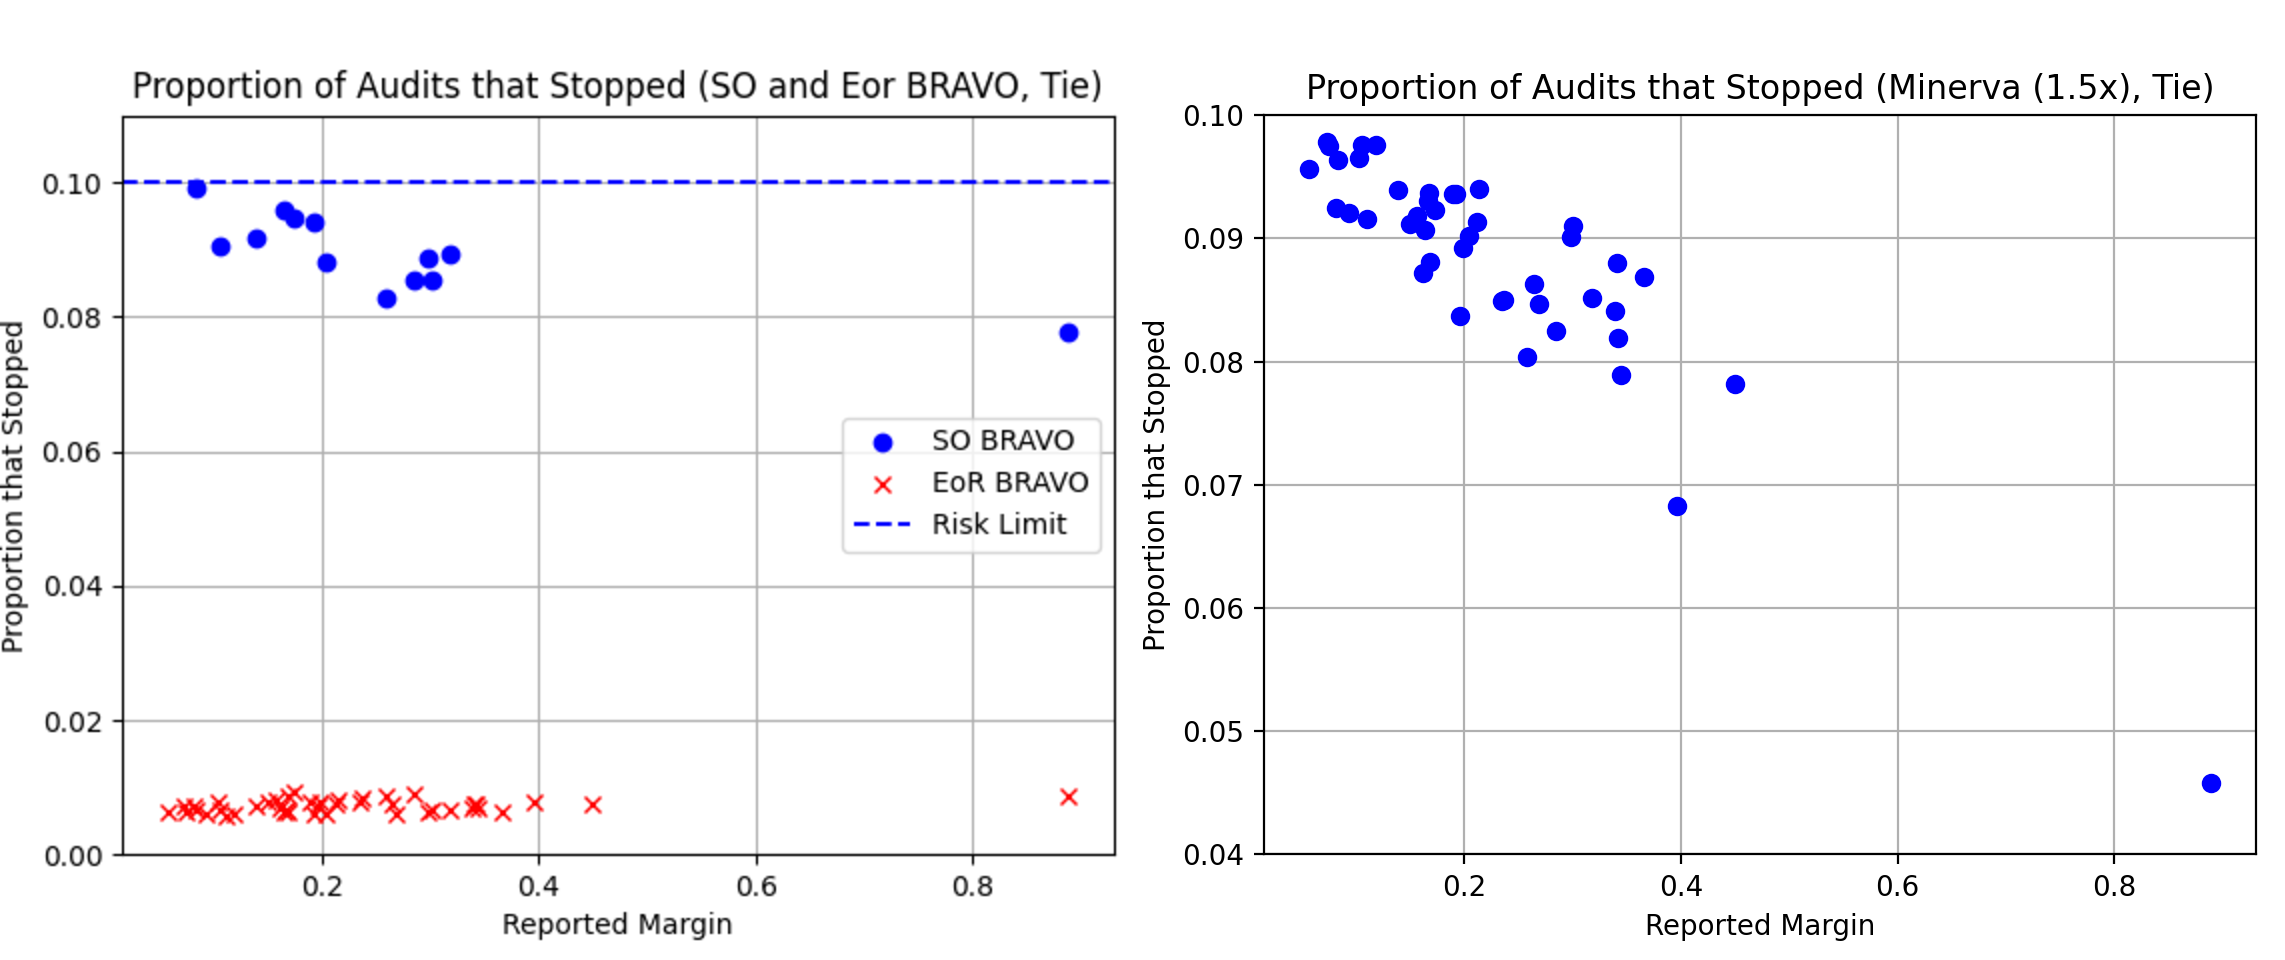
\includegraphics[width=\textwidth]{both_risk_plots.png}
\caption{The left hand plot shows the fraction of EoR \BRAVO audits (all states with margins at least $0.05$) and SO \BRAVO audits (the 13 states for which our simulations are complete so far) that stopped in any of the $5$ rounds when the underlying election was a tie. The right hand plot, for each state margin, shows the fraction of \Minerva audits with a round size multiple of $1.5$ that stopped in any of the $5$ rounds when the underlying election was a tie.}
\label{fig:risk}
%\end{centering}
\end{figure}
%
\end{block}

%\begin{block}{more}
%We present measures of stopping probability in the $j^{th}$ round of the audit, given that the underlying election is as announced.
%%%\begin{definition}[Stopping Probability]
%\heading{Definition: Stopping Probability}
%The stopping probability $S_j$ of an audit $\mathcal{A}$ in round $j$ is 
%$$S_j(\mathcal{A})=\Pr[\mathcal{A}(X)=Correct ~in~round~j~\land \mathcal{A}(X) \neq Correct ~previously \mid H_a]$$
%%\end{definition}
%Experimentally, using our simulations, $S_j$ would be estimated by the fraction of audits that stop in round $j$. Note that $\sum _j S_j(\mathcal{A})=1$. We can also consider the cumulative stopping probability: 
%%\begin{definition}[Cumulative Stopping Probability]
%The cumulative stopping probability $C_j$ of an audit $\mathcal{A}$ in round $j$ is $C_j(\mathcal{A})= \sum_{i=1}^j S_j$
%%\end{definition}
%Experimentally, using our simulations, $C_j$ would be estimated by the fraction of audits that stop in or before round $j$. 
%%
%We are also interested in the probability that an audit will stop in round $j$ given that it did not stop earlier: 
%%\begin{definition}[Conditional Stopping Probability]
%The conditional stopping probability  of an audit $\mathcal{A}$ in round $j$ is 
%$$\chi_j (\mathcal{A})=\Pr[\mathcal{A}(X)=Correct ~in~round~j~\mid H_a \land \mathcal{A}(X) \neq Correct ~previously]$$
%%\end{definition}
%Experimentally, using our simulations, $\chi_j$ would be estimated by the ratio of the audits that stop in round $j$ to those that ``entered'' round $j$, i.e. those that did not stop before round $j$. 
%%
%We simulated audits for a risk limit of $10\%$ (as in \cite{bravo} and \cite{usenix_minerva}) using margins from the 2020 US Presidential election, limiting ourselves to pairwise margins for the two main candidates of $0.05$ or larger. 
%Note that both \BRAVO and \Minerva can be extended for multiple-candidate, multiple-winner plurality contests by performing pairwise tests between the winners and the losers\cite{RLA, arxiv_athena}. Therefore, the two candidate plurality contest is a general case, and these simulations provide insight for multiple-candidate and multiple-winner contests too.
%%Round sizes increase roughly proportional to the inverse
%square of the margin, so 
%smaller margins are computationally much more expensive to simulate.
%For each of these states, we simulated 
%$10,000=10^4$ audits assuming the underlying election was as announced ($H_a$),  
%and an additional $10,000=10^4$ audits assuming the underlying election was a tie ($H_0$). 
%  \end{block}


%  \begin{block}{A block containing a list}
%
%    Nam vulputate nunc felis, non condimentum lacus porta ultrices. Nullam sed
%    sagittis metus. Etiam consectetur gravida urna quis suscipit.
%
%    \begin{itemize}
%      \item \textbf{Mauris tempor} risus nulla, sed ornare
%      \item \textbf{Libero tincidunt} a duis congue vitae
%      \item \textbf{Dui ac pretium} morbi justo neque, ullamcorper
%    \end{itemize}
%
%    Eget augue porta, bibendum venenatis tortor.
%
%  \end{block}
%
%  \begin{alertblock}{A highlighted block}
%
%    This block catches your eye, so \textbf{important stuff} should probably go
%%    here.
%%
%%%    Curabitur eu libero vehicula, cursus est fringilla, luctus est. Morbi
%%    consectetur mauris quam, at finibus elit auctor ac. Aliquam erat volutpat.
%%%    Aenean at nisl ut ex ullamcorper eleifend et eu augue. Aenean quis velit
%    tristique odio convallis ultrices a ac odio.
%
%    \begin{itemize}
%      \item \textbf{Fusce dapibus tellus} vel tellus semper finibus. In
%        consequat, nibh sed mattis luctus, augue diam fermentum lectus.
%      \item \textbf{In euismod erat metus} non ex. Vestibulum luctus augue in
%        mi condimentum, at sollicitudin lorem viverra.
%      \item \textbf{Suspendisse vulputate} mauris vel placerat consectetur.
%        Mauris semper, purus ac hendrerit molestie, elit mi dignissim odio, in
%        suscipit felis sapien vel ex.
%    \end{itemize}
%
%    Aenean tincidunt risus eros, at gravida lorem sagittis vel. Vestibulum ante
%    ipsum primis in faucibus orci luctus et ultrices posuere cubilia Curae.
%
%  \end{alertblock}

\end{column}

\separatorcolumn

\begin{column}{\colwidth}

  \begin{block}{Stopping Probability}

We are also interested in the probability that an audit will stop in round $j$ given that it did not stop earlier: 
%\begin{definition}[Conditional Stopping Probability]
The conditional stopping probability  of an audit $\mathcal{A}$ in round $j$ is 
$$\chi_j (\mathcal{A})=\Pr[\mathcal{A}(X)=Correct ~in~round~j~\mid H_a \land \mathcal{A}(X) \neq Correct ~previously]$$
%\end{definition}
Experimentally, using our simulations, $\chi_j$ would be estimated by the ratio of the audits that stop in round $j$ to those that ``entered'' round $j$, i.e. those that did not stop before round $j$. 
%
%%%%%%%%%%%%%%%%%%%%%%%%%%%%%%%%%%%%%%%%%%%%%%%%%%%%%%%%%%%%%%%%%%%%%%%%%%%%%%%%%%%%%%%%%%%%%%%%%%%%%%%%%%%%%%%%%%%%%%%%%%%%%%%%%%%%%%%%
\begin{figure}[h]
\centering

\begin{minipage}{.49\textwidth}
\begin{centering}
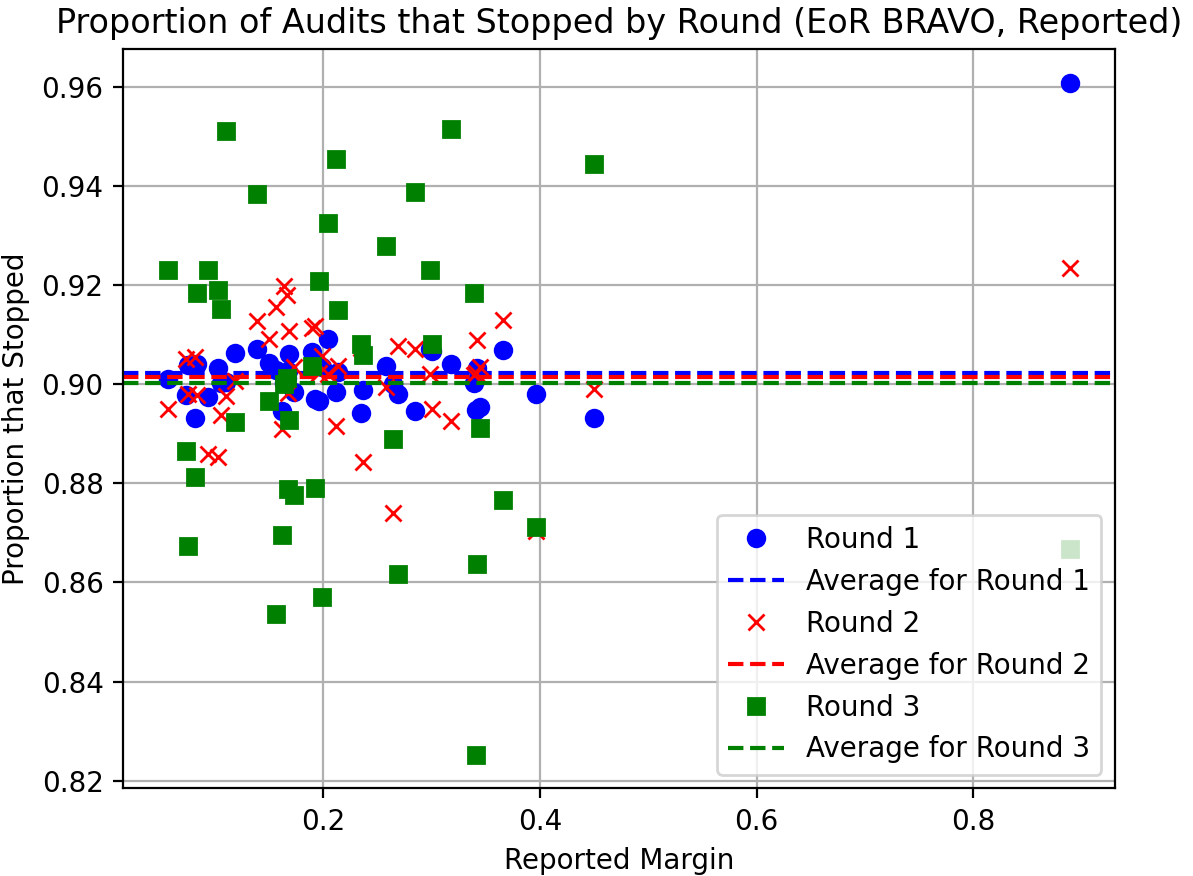
\includegraphics[width=1.0\textwidth]{eor_bravo_90perc_10^4_corrected/sprob_first_three_cropped.png}%\caption{This plot shows, for each state margin, when the underlying election is as announced, the number of EoR \BRAVO audits that stopped in the $j^{th}$ round, as a fraction of all EoR \BRAVO audits which had not yet stopped before the $j^{th}$ round for $j=1,2,3$ and $\chi_j=0.9$.}
\label{fig:eor_bravo_sprob}
\end{centering}\end{minipage}
\begin{minipage}{.49\textwidth}
\begin{centering}
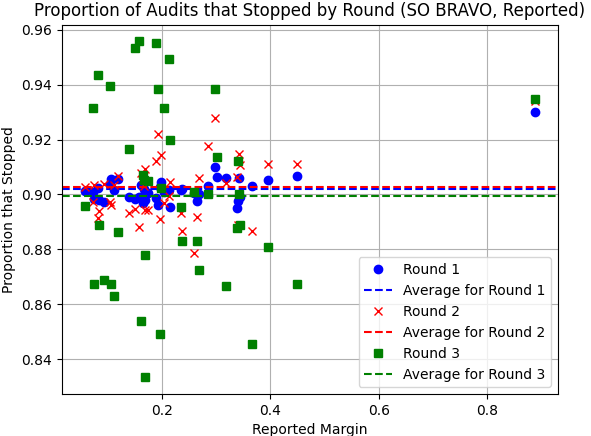
\includegraphics[width=1.0\textwidth]{so_bravo_90perc_10^4/sprob_first_three.png}%\caption{This plot shows, for each state margin, when the underlying election is as announced, the number of SO \BRAVO audits that stopped in the $j^{th}$ round,as a fraction of all SO \BRAVO audits which had not yet stopped before the $j^{th}$ round for $j=1,2,3$ and $\chi_j=0.9$.}
\label{fig:so_bravo_sprob}
\end{centering}
\end{minipage}
\caption{These plots show, for each state margin, when the underlying election is as announced, the number of audits that stopped in the $j^{th}$ round, as a fraction of all audits which had not yet stopped before the $j^{th}$ round for $j=1,2,3$ and $\chi_j=0.9$. The left shows EoR \BRAVO and the right shows SO \BRAVO.}
\end{figure}
%%%%%%%%%%%%%%%%%%%%%%%%%%%%%%%%%%%%%%%%%%%%%%%%%%%%%%%%%%%%%%%%%%%%%%%%%%%%%%%%%%%%%%%%%%%%%%%%%%%%%%%%%%%%%%%%%%%%%%%%%%%%%%%%%%%%%%%%
%\begin{figure}
%\begin{centering}
%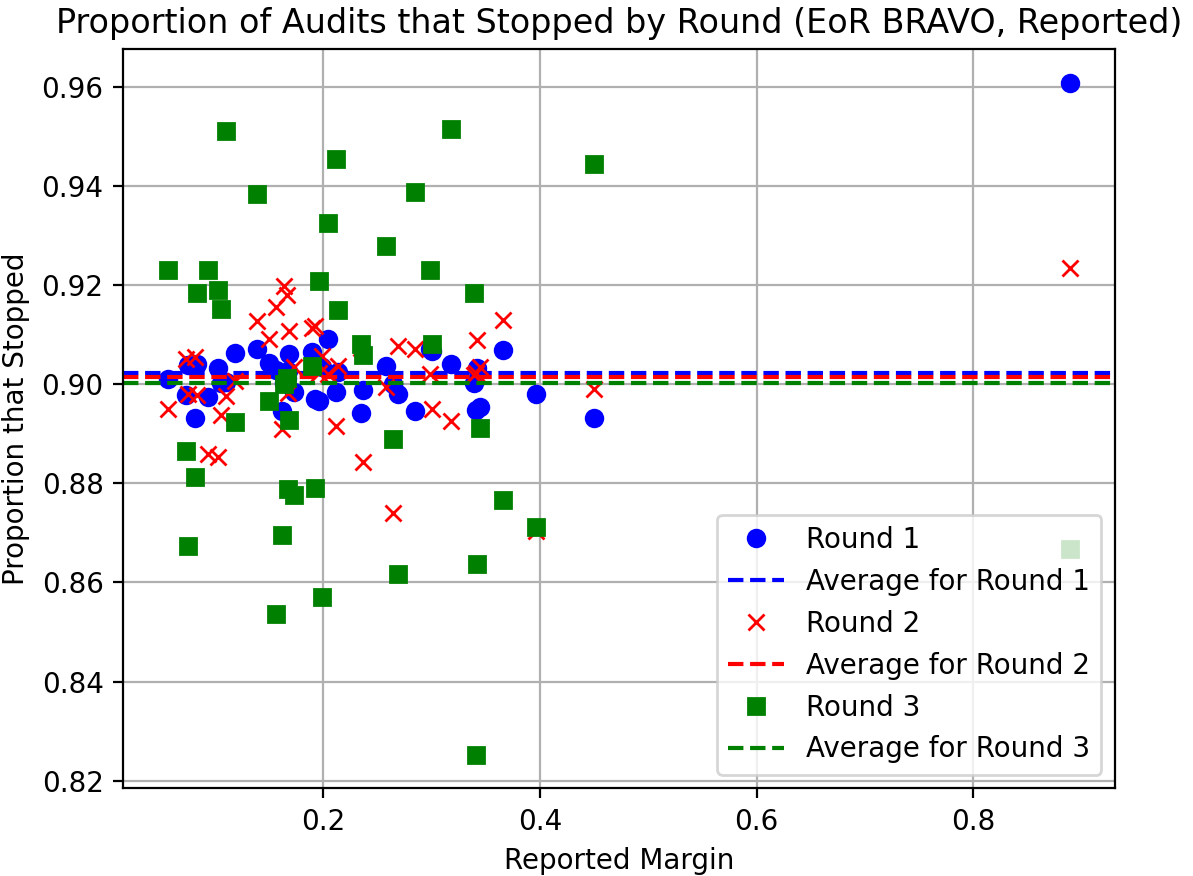
\includegraphics[width=0.6\textwidth]{eor_bravo_90perc_10^4_corrected/sprob_first_three_cropped.png}\caption{
%This plot shows, for each state margin, when the underlying election is as announced, the number of EoR \BRAVO audits that stopped in the $j^{th}$ round,
%as a fraction of all EoR \BRAVO audits which had not yet stopped before the $j^{th}$ round for $j=1,2,3$ and $S_1=0.9$.}
%%\label{fig:eor_bravo_sprob}
%\end{centering}
%\end{figure}
%
%\begin{figure}
%\begin{centering}
%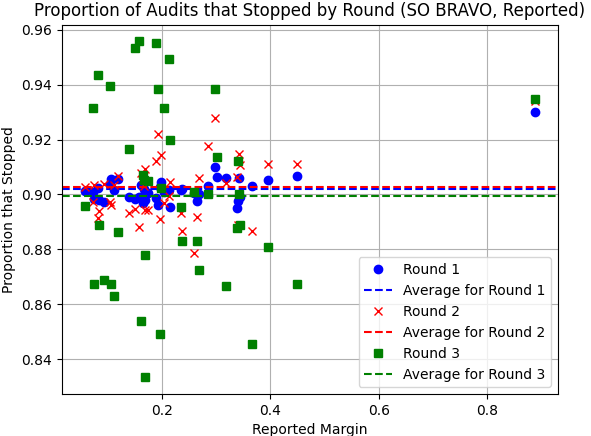
\includegraphics[width=0.6\textwidth]{so_bravo_90perc_10^4/sprob_first_three.png}\caption{
%This plot shows, for each state margin, when the underlying election is as announced, the number of SO \BRAVO audits that stopped in the $j^{th}$ round,
%as a fraction of all SO \BRAVO audits which had not yet stopped before the $j^{th}$ round for $j=1,2,3$ and $S_1=0.9$.}
%%\label{fig:so_bravo_sprob}
%\end{centering}
%\end{figure}
%
\begin{figure}[h]
\centering

\begin{minipage}{.49\textwidth}
%\begin{figure}
\begin{centering}
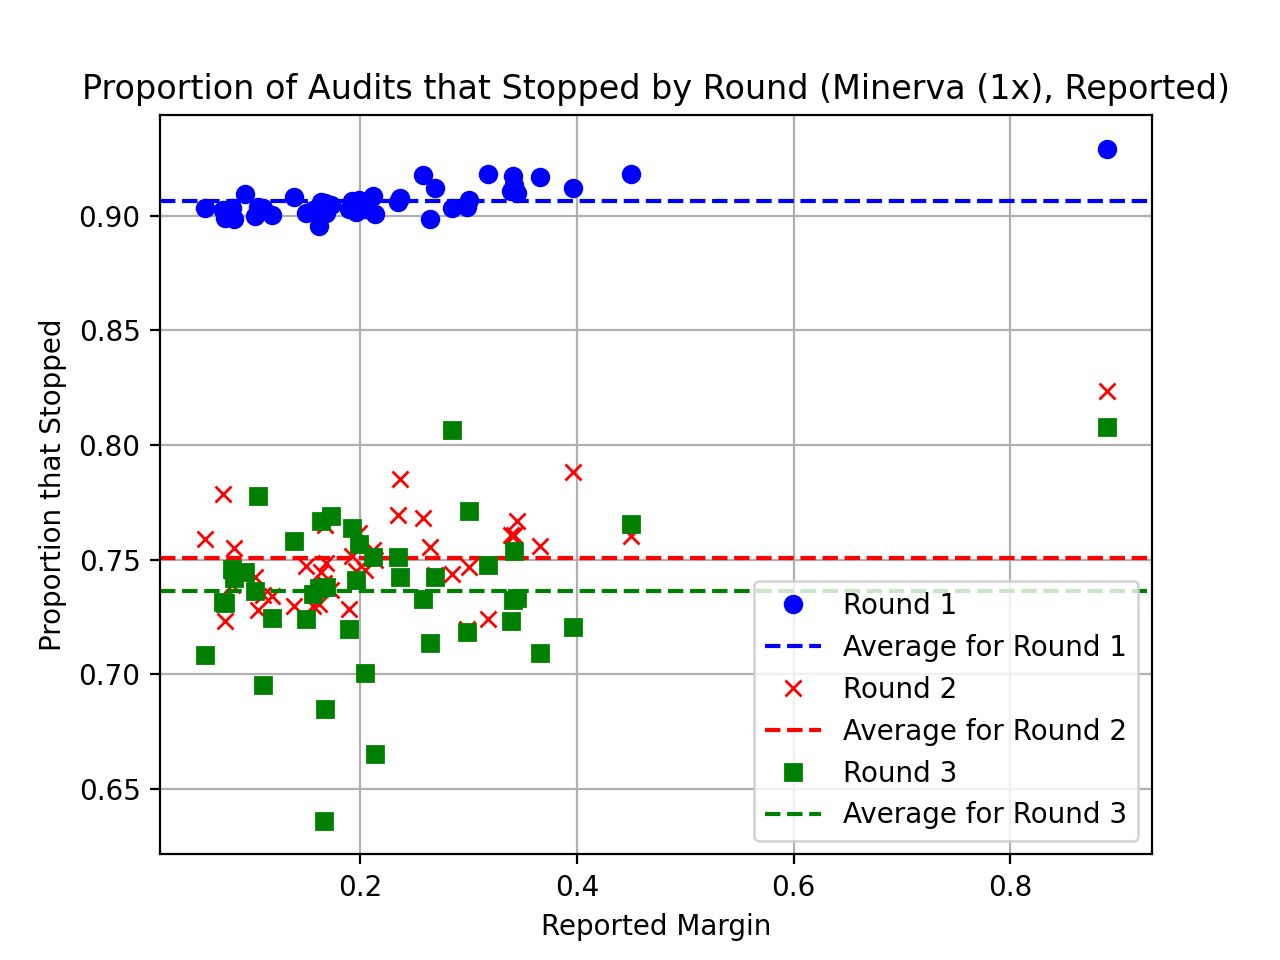
\includegraphics[width=1\textwidth]{minerva_multiround_1x_10^4/sprobs_first_three.png}
%\caption{This plot shows, for each state margin, when the underlying election is as announced, the number of \Minerva audits that stopped in the $j^{th}$ round, as a fraction of all \Minerva audits which had not yet stopped before the $j^{th}$ round for $j=1,2,3$, round size multiple of $1.0$ and $\chi_1=0.9$.}
\label{fig:minerva1_sprob}
\end{centering}
%\end{figure}
\end{minipage}
\begin{minipage}{.49\textwidth}
%\begin{figure}
\begin{centering}
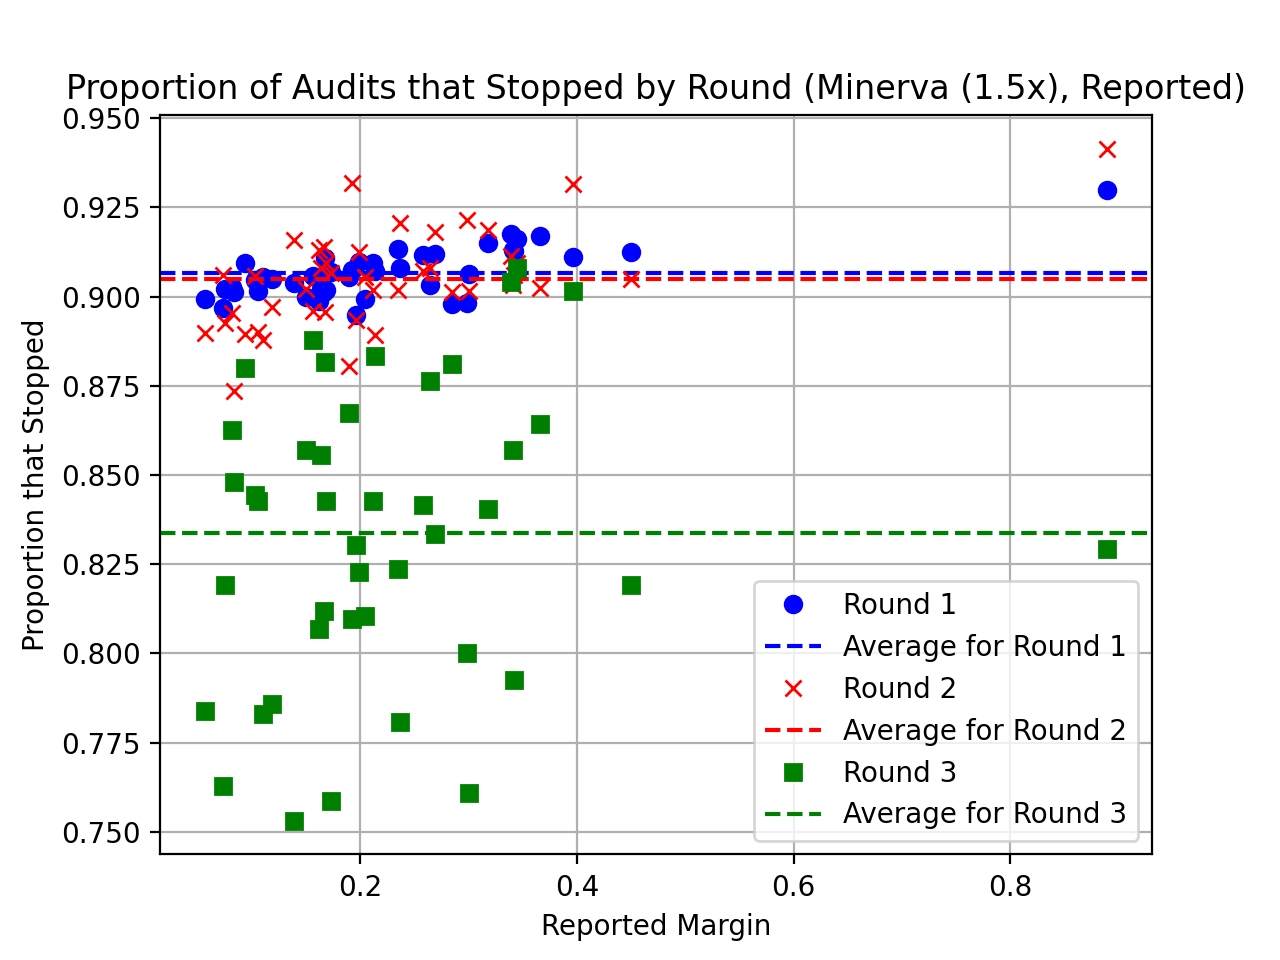
\includegraphics[width=1\textwidth]{minerva_multiround_1p5x_10^4/sprobs_first_three.png}
%\caption{This plot shows, for each state margin, when the underlying election is as announced, the number of \Minerva audits that stopped in the $j^{th}$ round, as a fraction of all \Minerva audits which had not yet stopped before the $j^{th}$ round for $j=1,2,3$, round size multiple of $1.5$ and $\chi_1=0.9$.}
\label{fig:minerva1p5_sprob}
\end{centering}
%\end{figure}
\end{minipage}
\caption{These plots show, for each state margin, when the underlying election is as announced, the number of \Minerva audits that stopped in the $j^{th}$ round, as a fraction of all \Minerva audits which had not yet stopped before the $j^{th}$ round for $j=1,2,3$. The left shows \Minerva with the round schedule obtained by $\chi_1=0.9$ and round size multiple $1.5$.}
\end{figure}

We can perform a similar study for a first round size with $\chi_1=0.25$. 
See Figure~\ref{fig:minerva_25} for an example, \Minerva with round mutiplier $1.5$. 

\begin{figure}
\begin{centering}
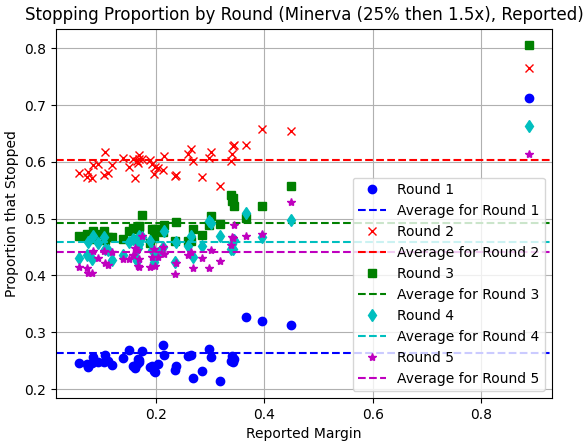
\includegraphics[width=0.6\textwidth]{minerva25percthen1p5_sprob.png}
\caption{This plot shows, for each state margin, when the underlying election is as announced, the number of \Minerva audits that stopped in the $j^{th}$ round,
as a fraction of all \Minerva audits which had not yet stopped before the $j^{th}$ round for $j=1,2,3$, round size multiple of $1.5$ and $\chi_1 = 0.25$.}
\label{fig:minerva_25}
\end{centering}
\end{figure}

  \end{block}

%  \begin{block}{Fusce aliquam magna velit}
%
%    Et rutrum ex euismod vel. Pellentesque ultricies, velit in fermentum
%    vestibulum, lectus nisi pretium nibh, sit amet aliquam lectus augue vel
%    velit. Suspendisse rhoncus massa porttitor augue feugiat molestie. Sed
%    molestie ut orci nec malesuada. Sed ultricies feugiat est fringilla
%    posuere.
%
%    \begin{figure}
%      \centering
%      \begin{tikzpicture}
%        \begin{axis}[
%            scale only axis,
%            no markers,
%            domain=0:2*pi,
%            samples=100,
%            axis lines=center,
%            axis line style={-},
%            ticks=none]
%          \addplot[red] {sin(deg(x))};
%          \addplot[blue] {cos(deg(x))};
%        \end{axis}
%      \end{tikzpicture}
%      \caption{Another figure caption.}
%    \end{figure}
%
%  \end{block}
%
%  \begin{block}{Nam cursus consequat egestas}
%
%    Nulla eget sem quam. Ut aliquam volutpat nisi vestibulum convallis. Nunc a
%    lectus et eros facilisis hendrerit eu non urna. Interdum et malesuada fames
%    ac ante \textit{ipsum primis} in faucibus. Etiam sit amet velit eget sem
%    euismod tristique. Praesent enim erat, porta vel mattis sed, pharetra sed
%    ipsum. Morbi commodo condimentum massa, \textit{tempus venenatis} massa
%    hendrerit quis. Maecenas sed porta est. Praesent mollis interdum lectus,
%    sit amet sollicitudin risus tincidunt non.
%
%    Etiam sit amet tempus lorem, aliquet condimentum velit. Donec et nibh
%    consequat, sagittis ex eget, dictum orci. Etiam quis semper ante. Ut eu
%    mauris purus. Proin nec consectetur ligula. Mauris pretium molestie
%    ullamcorper. Integer nisi neque, aliquet et odio non, sagittis porta justo.
%
%    \begin{itemize}
%      \item \textbf{Sed consequat} id ante vel efficitur. Praesent congue massa
%        sed est scelerisque, elementum mollis augue iaculis.
%        \begin{itemize}
%          \item In sed est finibus, vulputate
%            nunc gravida, pulvinar lorem. In maximus nunc dolor, sed auctor eros
%            porttitor quis.
%          \item Fusce ornare dignissim nisi. Nam sit amet risus vel lacus
%            tempor tincidunt eu a arcu.
%          \item Donec rhoncus vestibulum erat, quis aliquam leo
%            gravida egestas.
%        \end{itemize}
%      \item \textbf{Sed luctus, elit sit amet} dictum maximus, diam dolor
%        faucibus purus, sed lobortis justo erat id turpis.
%      \item \textbf{Pellentesque facilisis dolor in leo} bibendum congue.
%        Maecenas congue finibus justo, vitae eleifend urna facilisis at.
%    \end{itemize}
%    
%    Nulla eget sem quam. Ut aliquam volutpat nisi vestibulum convallis. Nunc a
%    lectus et eros facilisis hendrerit eu non urna. Interdum et malesuada fames
%    ac ante \textit{ipsum primis} in faucibus. Etiam sit amet velit eget sem
%    euismod tristique. Praesent enim erat, porta vel mattis sed, pharetra sed
%    ipsum. Morbi commodo condimentum massa, \textit{tempus venenatis} massa
%    hendrerit quis. Maecenas sed porta est. Praesent mollis interdum lectus,
%    sit amet sollicitudin risus tincidunt non.
%  \end{block}
%
\end{column}

\separatorcolumn

\begin{column}{\colwidth}


\begin{block}{Number of Ballots}
\begin{itemize}
\item
The number of ballots sampled is one crude measure of the workload of an audit.
To keep the costs of RLAs low, audits should be designed to stop with as few ballots as possible.
\item
The following plots show the probability of stopping as a function of the average number of ballots
sampled by round in our simulations.
\end{itemize}

\begin{figure}[h]
\centering
\begin{minipage}{.49\textwidth}
\begin{centering}
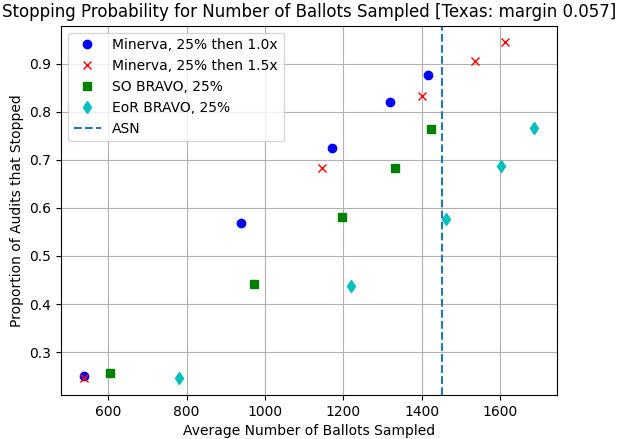
\includegraphics[width=1\textwidth]{texas25.png}
%\caption{This plot shows the cumulative fraction of audits that stopped as a function of average number of sampled ballots for all four audits we studied, for the state of Texas, margin $0.057$, and first round stopping probability $S_1=0.25$.}
\label{fig:texas_25}
\end{centering}
\end{minipage}
\begin{minipage}{.49\textwidth}
\begin{centering}
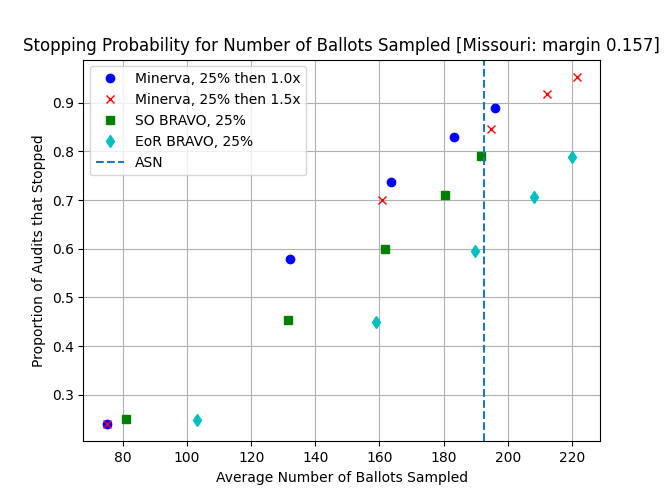
\includegraphics[width=1\textwidth]{missouri25.png}
%\caption{This plot shows the cumulative fraction of audits that stopped as a function of average number of sampled ballots for all four audits we studied, for the state of Missouri, margin $0.157$, and first round stopping probability $S_1=0.25$.}
\label{fig:missouri_25}
\end{centering}
\end{minipage}
\caption{These plots show the cumulative fraction of audits that stopped as a function of average number of sampled ballots for all four audits we studied, for the states of Texas with margin $.057$ (left) and Missouri with margin $0.157$ (right), both with first round stopping probability $\chi_1=0.25$.}
\end{figure}

\begin{figure}[h]
\centering
\begin{minipage}{.49\textwidth}
\begin{centering}
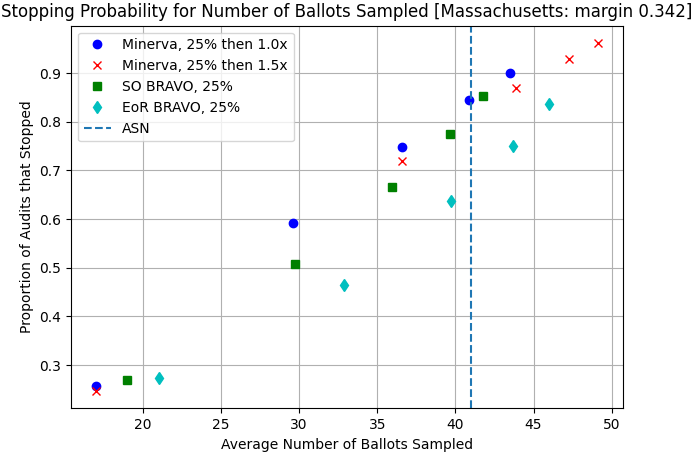
\includegraphics[width=1\textwidth]{massachusetts25.png}
%\caption{This plot shows the cumulative fraction of audits that stopped as a function of average number of sampled ballots for all four audits we studied, for the state of Massachusetts, margin $0.342$, and first round stopping probability $\chi_1=0.25$.}
\label{fig:mass_25}
\end{centering}
\end{minipage}
\begin{minipage}{.49\textwidth}
\begin{centering}
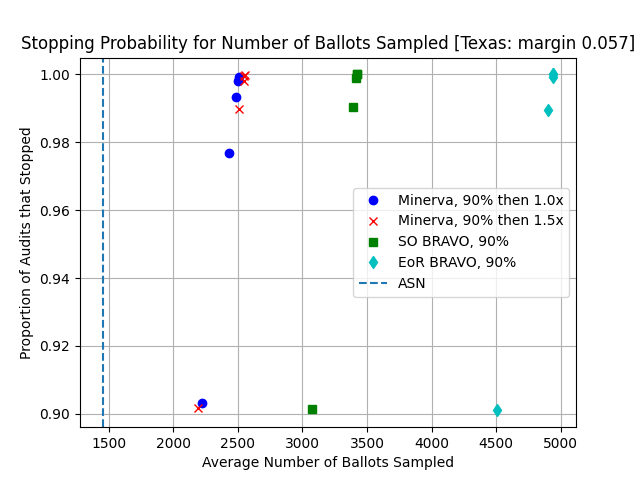
\includegraphics[width=1\textwidth]{texas90.png}
%\caption{This plot shows the cumulative fraction of audits that stopped as a function of average number of sampled ballots for all four audits we studied, for the state of Texas, margin $0.057$, and first round stopping probability $\chi_1=0.9$.}
\label{fig:texas_90}
\end{centering}
\end{minipage}
\caption{These plots show the cumulative fraction of audits that stopped as a function of average number of sampled ballots for all four audits we studied, for the states Massachusetts (left) with margin $0.342$ and $\chi_1=0.25$ and Texas (right) with margin $0.057$ and $\chi_1=0.9$.}
\end{figure}

For $\chi_1=0.25$, the ratio of first round size of EoR \BRAVO to \Minerva is $1.45$, $1.37$, $1.23$ for states Texas, Missouri and Massachusetts, and margins $0.057$, $0.157$ and $0.342$ respectively. This may be compared to $2.03$, $1.99$ and $1.8$ respectively for $\chi_1=0.9$. Similarly, for $\chi_1=0.25$, the ratio of first round size of SO \BRAVO to \Minerva is $1.13$, $1.08$, $1.12$ for states Texas, Missouri and Massachusetts, and margins $0.057$, $0.157$ and $0.342$ respectively. This may be compared to $1.38$, $1.38$ and $1.30$ respectively for $\chi_1=0.9$. 


\end{block}


\begin{block}{Modeling Workload}

\emph{I initially wrote this section since I'd really like to have some evidence that for certain workload parameters, we see an optimal
number of rounds greater than 1 with Providence. I am working on that code now.}

\BRAVO requires the smallest expected number of ballots when ballots are drawn one at a time and the (true) underlying election is as announced. 
In real audits, election officials draw ballots in rounds because their is some overhead with each round (e.g. opening ballot boxes).
Therefore a more sophisticated workload model has a per ballot cost $c_b$ and a per round cost $c_r$. 
Let $n$ be the number of ballots sampled and $j$ be the number of rounds. Then the cost $C$ is given by 
$$C(n,j) = c_b\cdot n + c_r\cdot j,$$
and depending on the ratio between $c_b$ and $c_r$, we should expect that certain round schedules
achieve lower expected cost.
\end{block}

%  \begin{block}{A block containing some math}
%
%    Nullam non est elit. In eu ornare justo. Maecenas porttitor sodales lacus,
%    ut cursus augue sodales ac.
%
%    $$
%    \int_{-\infty}^{\infty} e^{-x^2}\,dx = \sqrt{\pi}
%    $$
%
%    Interdum et malesuada fames $\{1, 4, 9, \ldots\}$ ac ante ipsum primis in
%    faucibus. Cras eleifend dolor eu nulla suscipit suscipit. Sed lobortis non
%    felis id vulputate.
%
%    \heading{A heading inside a block}
%
%    Praesent consectetur mi $x^2 + y^2$ metus, nec vestibulum justo viverra
%    nec. Proin eget nulla pretium, egestas magna aliquam, mollis neque. Vivamus
%    dictum $\mathbf{u}^\intercal\mathbf{v}$ sagittis odio, vel porta erat
%    congue sed. Maecenas ut dolor quis arcu auctor porttitor.
%
%    \heading{Another heading inside a block}
%
%    Sed augue erat, scelerisque a purus ultricies, placerat porttitor neque.
%    Donec $P(y \mid x)$ fermentum consectetur $\nabla_x P(y \mid x)$ sapien
%    sagittis egestas. Duis eget leo euismod nunc viverra imperdiet nec id
%    justo.
%
%  \end{block}
%
%  \begin{block}{Nullam vel erat at velit convallis laoreet}
%
%%    Class aptent taciti sociosqu ad litora torquent per conubia nostra, per
%    inceptos himenaeos. Phasellus libero enim, gravida sed erat sit amet,
%    scelerisque congue diam. Fusce dapibus dui ut augue pulvinar iaculis.
%%
%    \begin{table}
%      \centering
%%      \begin{tabular}{l r r c}
%        \toprule
%%        \textbf{First column} & \textbf{Second column} & \textbf{Third column} & \textbf{Fourth} \\
%        \midrule
%        Foo & 13.37 & 384,394 & $\alpha$ \\
%%        Bar & 2.17 & 1,392 & $\beta$ \\
%        Baz & 3.14 & 83,742 & $\delta$ \\
%        Qux & 7.59 & 974 & $\gamma$ \\
%%        \bottomrule
%      \end{tabular}
%      \caption{A table caption.}
%%    \end{table}
%
%    Donec quis posuere ligula. Nunc feugiat elit a mi malesuada consequat. Sed
%%    imperdiet augue ac nibh aliquet tristique. Aenean eu tortor vulputate,
%    eleifend lorem in, dictum urna. Proin auctor ante in augue tincidunt
%%    tempor. Proin pellentesque vulputate odio, ac gravida nulla posuere
%    efficitur. Aenean at velit vel dolor blandit molestie. Mauris laoreet
%%    commodo quam, non luctus nibh ullamcorper in. Class aptent taciti sociosqu
%    ad litora torquent per conubia nostra, per inceptos himenaeos.
%
%    Nulla varius finibus volutpat. Mauris molestie lorem tincidunt, iaculis
%%    libero at, gravida ante. Phasellus at felis eu neque suscipit suscipit.
%    Integer ullamcorper, dui nec pretium ornare, urna dolor consequat libero,
%    in feugiat elit lorem euismod lacus. Pellentesque sit amet dolor mollis,
%%    auctor urna non, tempus sem.
%
%%  \end{block}

\end{column}

\separatorcolumn

\begin{column}{\colwidth}
\begin{block}{Providence}

\begin{itemize}
\item
The efficiency of \Minerva is great, but it lacks the flexibility of \BRAVO in choosing round sizes based on previous samples.
\item
\Prov is our novel RLA which has the efficiency of \Minerva and the flexibility of \BRAVO.
\item For alternative hypothesis $H_a$ that the election is truly as announced and null
hypothesis $H_0$ that the true election is a tie, \BRAVO has the stopping condition that
for $k$ cumulative ballots for the winner and $n$ cumulative sampled ballots,
$$\sigma(k,n,p_a,p_0) \triangleq \frac{\Pr[K=k\mid H_a, n]}{\Pr[K=k\mid H_0, n]}\ge \frac{1}{\alpha}.$$
\item \Minerva has the stopping condition that in round $j$ with cumulative winner ballots $k_j$ and round sizes $\bar n_j = n_1,n_2,\ldots,n_j$
$$\tau_j(k_j,\bar n_j,p_a,p_0) \triangleq \frac{\Pr[K_j\ge k_j \wedge \mathcal{A}_{i<j}(X)\neq Correct \mid H_a, \bar n_j]}{\Pr[K_j\ge k_j \wedge \mathcal{A}_{i<j}(X)\neq Correct \mid H_0, \bar n_j]}\ge \frac{1}{\alpha}.$$ Testing this stopping condition requires computationaly expensive convolutions.
\item The \Prov stopping condition uses ideas from both \BRAVO and \Minerva and requires no convolution to test:
$$\omega_j(k_{j-1},k_j,n_{j-1},n_j,p_a,p_0)\triangleq \sigma(k_{j-1},n_{j-1},p_a,p_0)\cdot \tau_1(k_j,n_j,p_a,p_0) \ge \frac{1}{\alpha}.$$ 

\end{itemize}

\heading {Resistance against an adversary} 
If adversary $\mathcal{A}$ has knowledge of previous samples and chooses round size $n_j$ in round $j$, 
\Prov is still risk-limiting. Proof of this and the RLA property of \Prov are currently being revised for submission.

\heading {\Prov pilot}
In February 2022, The Rhode Island Board of Elections hosted a public pilot \Prov RLA which passed 
in the first round.

\begin{figure}
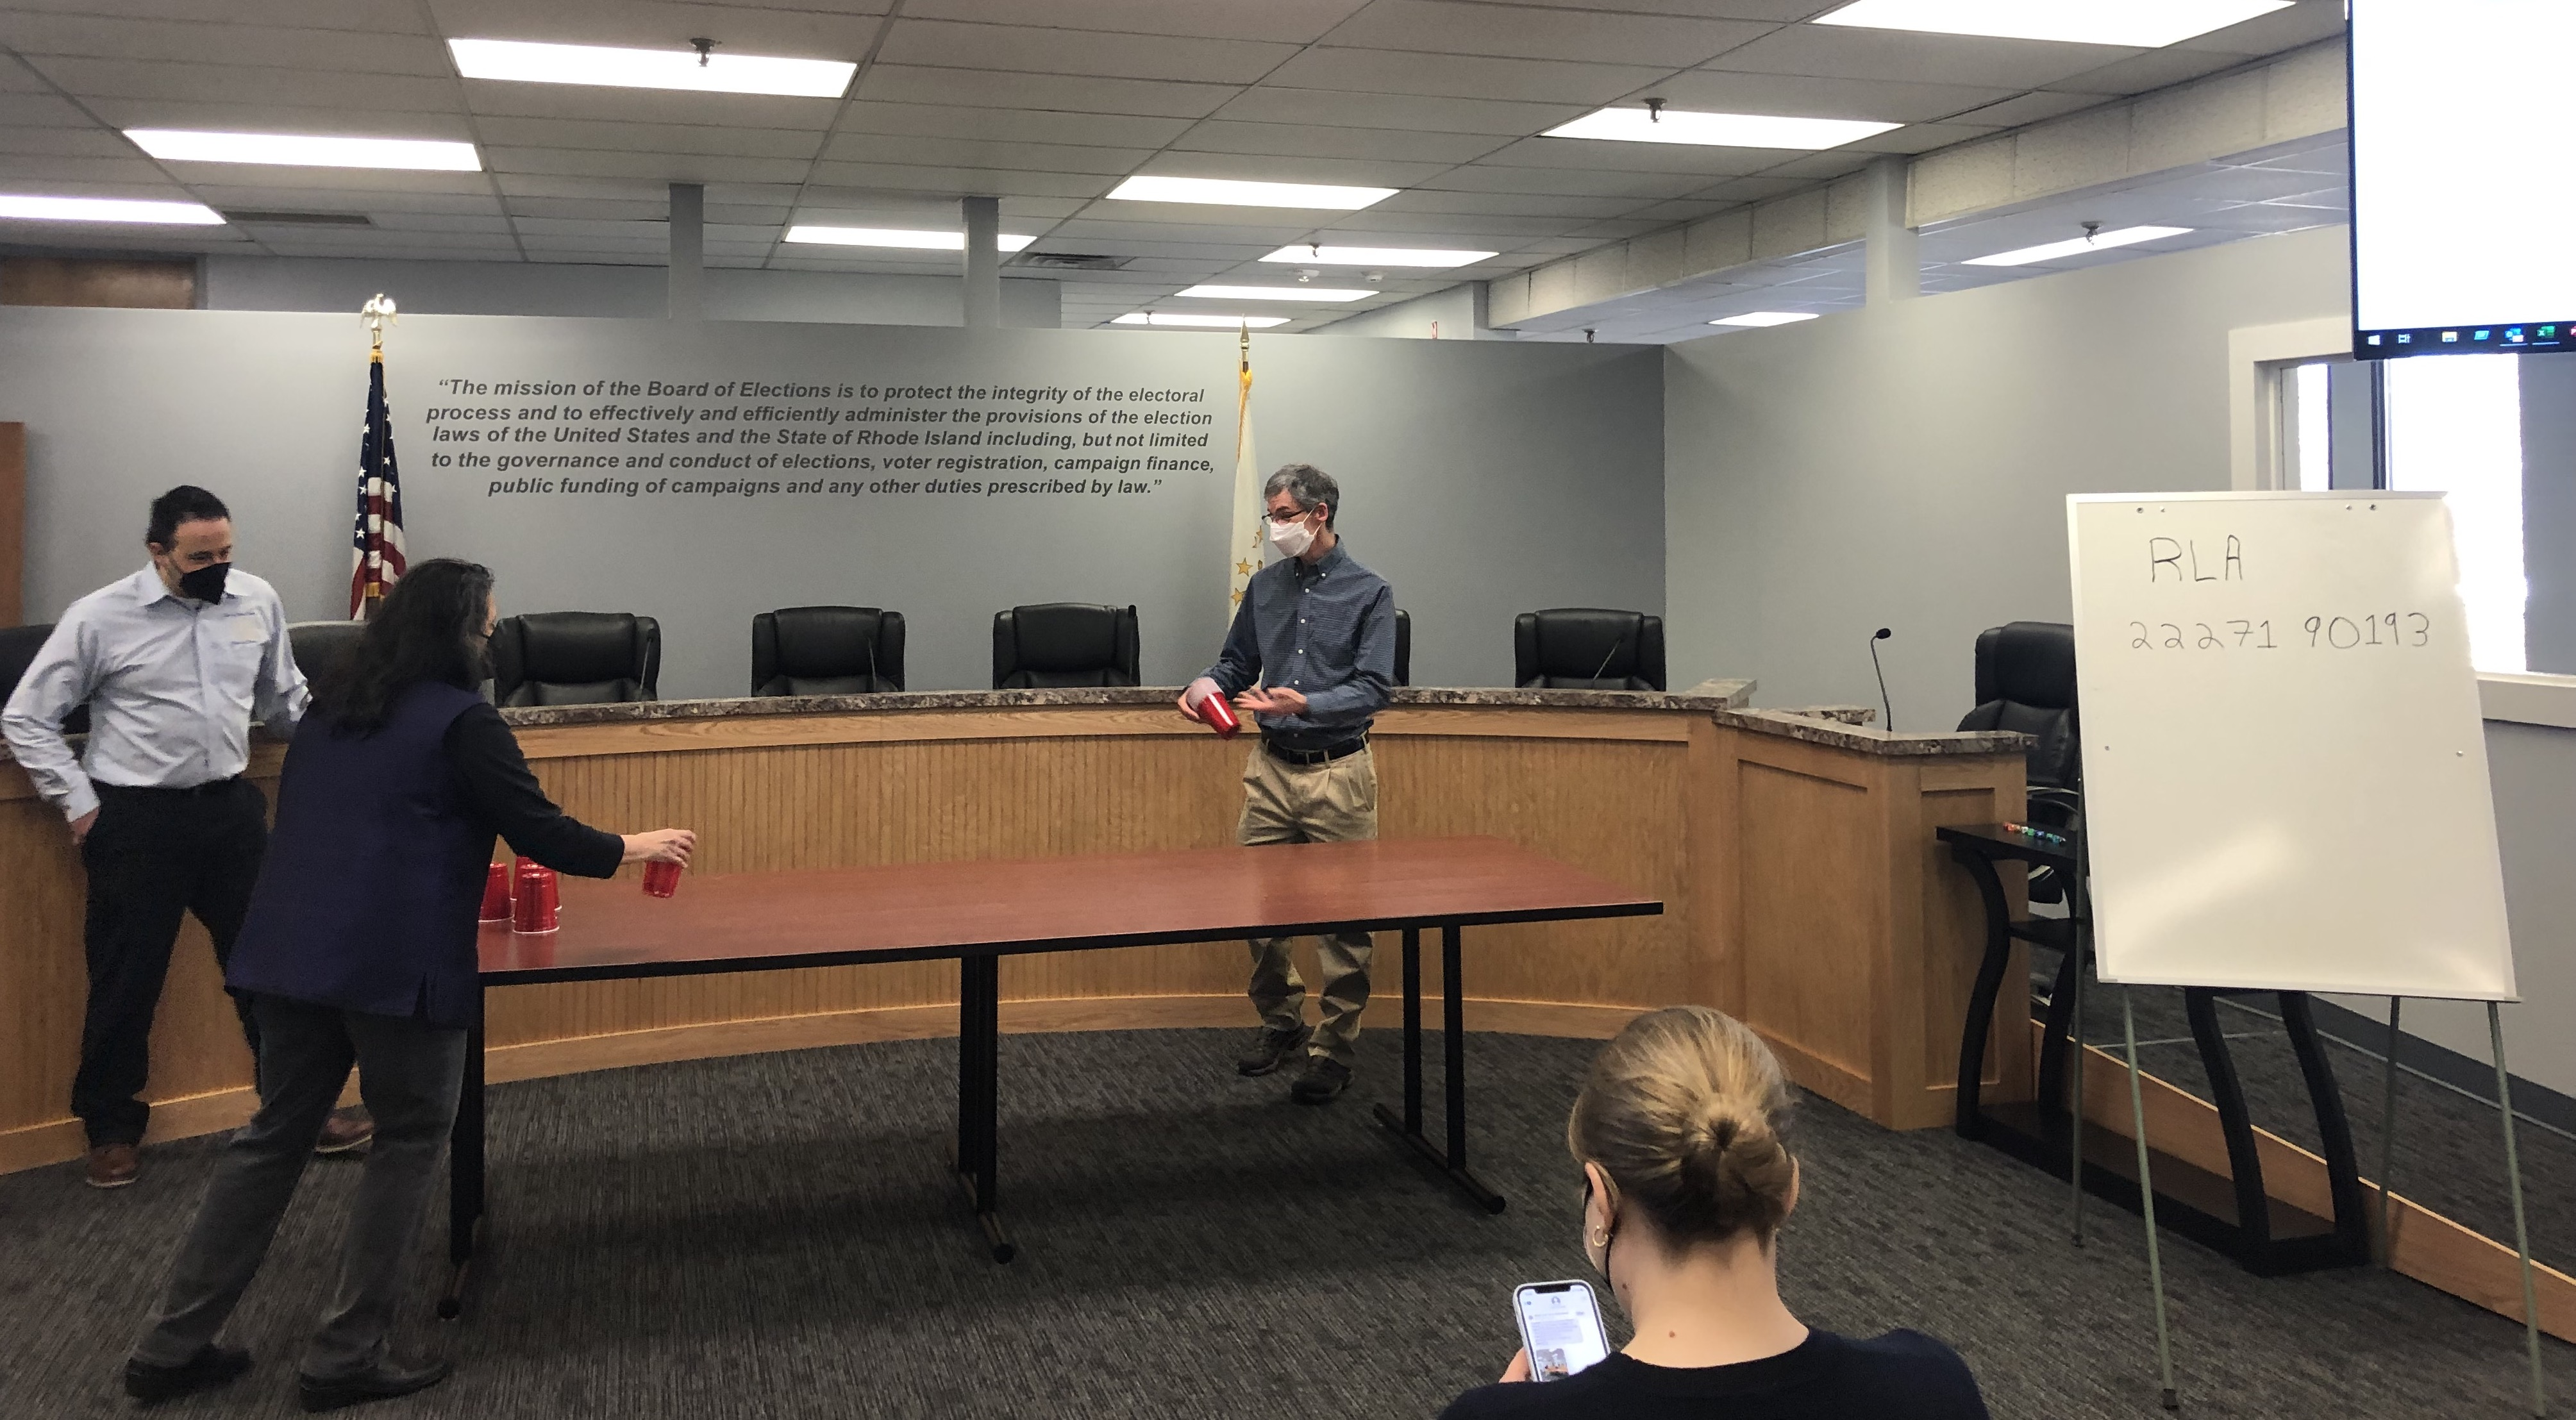
\includegraphics[width=1.0\textwidth]{dice.jpg}
\caption{Professor Vora tosses her random-seed-generating 10-sided die, in a roll she dedicated to election officials everywhere.}
\end{figure}

\end{block}

\begin{block}{Simulations}

\emph{Need to fill in simulation results here. I am thinking (a) risk simulations as evidence that \Prov is an RLA, and (b) number of ballot results if I get them done quickly enough.}

Simulations are currently running to explore the risk, stopping probability, and number of ballots used by \Prov.

\end{block}



  \begin{block}{References}

    %\nocite{*}
    %\footnotesize{\bibliographystyle{plain}\bibliography{audits}}
    \bibliographystyle{splncs04}
    %\bibliographystyle{plain}
    \bibliography{audits}
    \emph{Having some latex trouble here, but should include r2b2, the recent simulations paper, bravo paper, athena paper, ...}

  \end{block}


\end{column}

\separatorcolumn

\end{columns}

\end{frame}

\end{document}

